\documentclass[conference]{IEEEtran}
\IEEEoverridecommandlockouts
\usepackage{cite}
\usepackage{amsmath,amssymb}
\usepackage{graphicx}
\usepackage{textcomp}
\usepackage{xcolor}
\usepackage[T1]{fontenc}
\usepackage[utf8]{inputenc}
\usepackage{url}
\def\BibTeX{{\rm B\kern-.05em{\sc i\kern-.025em b}\kern-.08em
    T\kern-.1667em\lower.7ex\hbox{E}\kern-.125emX}}
\begin{document}

\title{PACT: An Accountability Protocol for Deployed AI Systems, with Measured Limits on AI-Jury Adjudication}

\author{\IEEEauthorblockN{Saish Sanjay Shinde}
\IEEEauthorblockA{\textit{San Jos\'e State University} \\
San Jos\'e, CA, USA \\
saish.shinde@sjsu.edu}}

\maketitle

\begin{abstract}
Institutional oversight of AI rests on a weak foundation. Third-party evaluation, statutory record-keeping and proposals for verifiable limits on frontier development all presume an audit record. That record is produced and held by the operator of the system under audit. We present PACT, a protocol that makes deployed AI conduct non-repudiable and adjudicable among mutually distrusting parties. PACT separates a cheap evidence plane, consisting of per-agent hash-chained conduct logs whose Merkle checkpoints are cosigned by independent witnesses, from a small governance plane holding registries, challenges, verdicts and consequences. Conduct is policed recursively: watchdog agents file challenges, diversity-constrained juries of evaluator models vote by commit--reveal and humans hold final appeal. Jurors are themselves covered by the mechanism. We built a reference implementation that runs the full loop at 122 \textmu{}s per covered action and costs 13.3 B of shared ledger per query. In it, one action in 100,000 remains provable to a witness-cosigned root through 22 hashes. Our central results are negative and were produced by that implementation against its own design. Auditing our own corpus against its policy clause found 11 of its 32 violation labels in conflict with the clause's live-credential qualifier; we adjudicated the conflict and corrected the labels in place, and every number is reported under both the authored and the corrected labels, the corrected figure primary. What survives every labelling regime and both prompt framings we tried is a pair of invariants rather than any point value. First, aggregation buys containment and never accuracy: an asymmetric voting rule holds containment of true violations at 0.905 (95\% CI [0.762, 1.000]) where the plain two-thirds rule leaks 71.4\% of them (0.286 [0.095, 0.476], disjoint intervals), yet on a nineteen-juror panel spanning nine vendors every voting rule --- two-thirds, simple majority, and the asymmetric rule itself --- scores below the best single juror under corrected labels in both framings. Second, juror errors correlate as judgment, not lineage: cross-vendor pairs are as correlated as within-vendor pairs in all six cuts we ran (difference 95\% CI contains zero in each), the panel-mean joint-error ratio exceeds independence in every bootstrap replicate under every regime --- its magnitude moving from 2.7$\times$ to 5.8$\times$ with labels and framing, a spread we report as a finding about the measurement itself --- and the items that defeat whole panels are exactly the ones pre-labelled contested. This agrees with concurrent findings on generic judge panels \cite{r39,r40}; we measure it where a verdict carries consequence and we change the protocol in response: the diversity constraint is restated as selection for measured complementarity and no auto-clear rests on juror agreement.
\end{abstract}

\begin{IEEEkeywords}
AI accountability, transparency logs, LLM-as-judge, distributed systems security, adjudication protocols, empirical evaluation
\end{IEEEkeywords}

\section{Introduction}

\begin{figure*}[t]
\centering
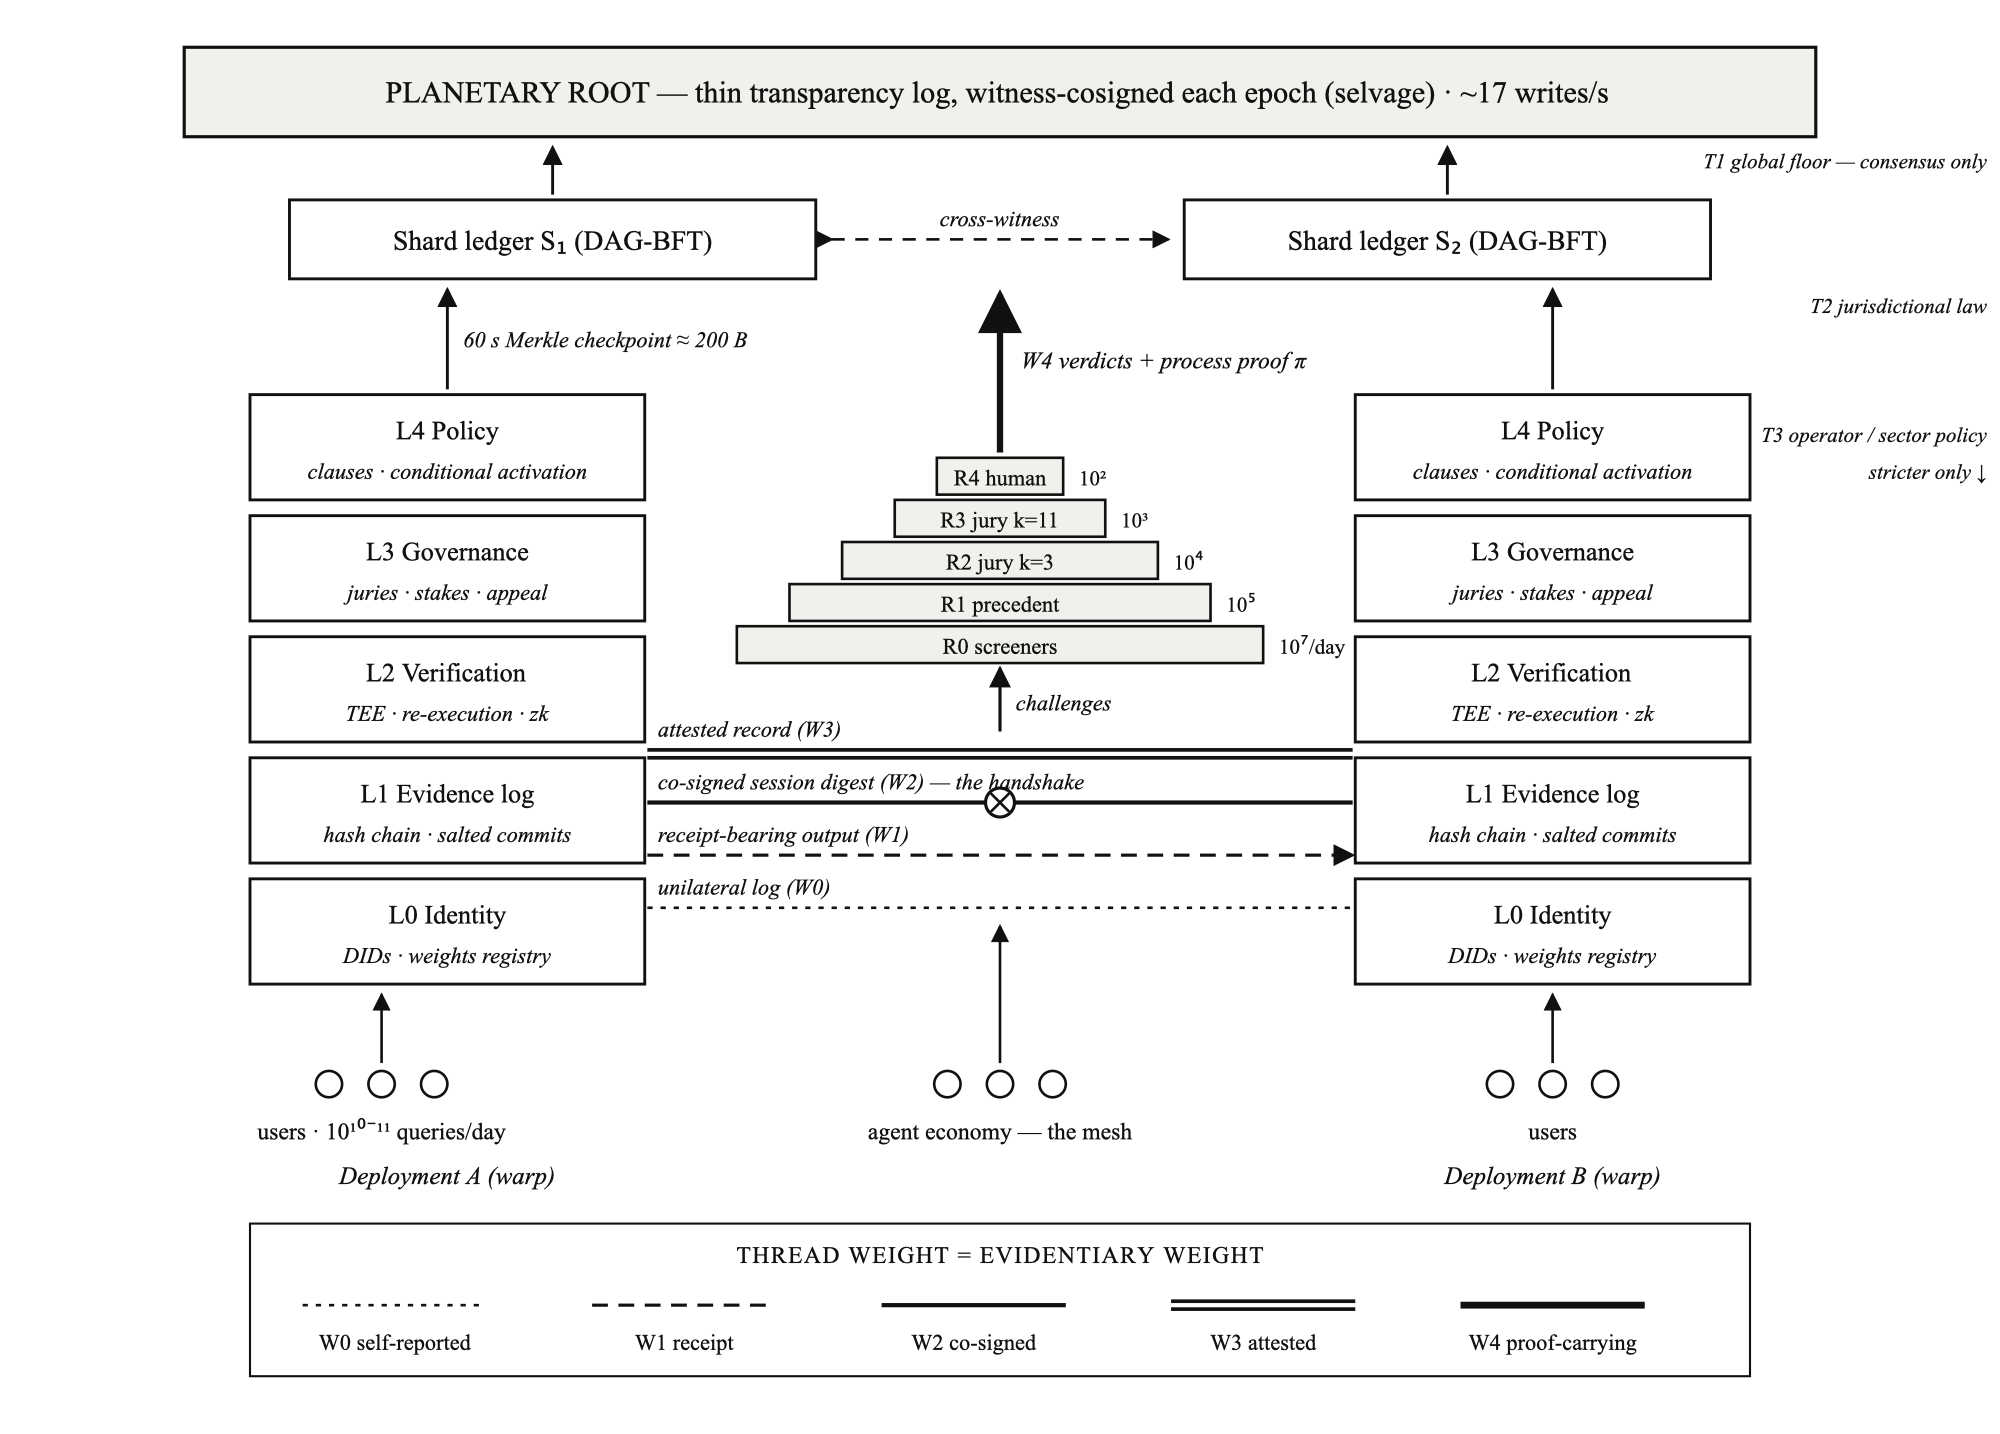
\includegraphics[width=\textwidth]{figs/loom.png}
\caption{The accountability loom. Vertical warp columns are per-deployment stacks;
horizontal weft threads are interaction evidence, drawn with thread weight proportional
to evidentiary class; the central funnel is the shuttle turning flagged threads into
verdicts; the witness-cosigned root is the selvage. The right-hand rail marks the three
policy tiers at their native altitude.}
\label{fig:loom}
\end{figure*}


Oversight of AI systems is acquiring an institutional layer faster than a technical one. Regulators impose record-keeping and incident-reporting duties on high-risk systems \cite{r18}, developers publish safety frameworks and invite external evaluation. Policy proposals call for verification arrangements spanning parties that do not trust one another. Every such mechanism presumes a trustworthy account of what an AI system did. In current practice that account is produced, stored and served by the operator of the system under audit, so the record is editable by the party it constrains.

Transparency logs solved the analogous problem for web certificates \cite{r1}, but detection-only machinery is insufficient here. AI oversight also needs a place to challenge recorded conduct, a procedure to adjudicate the challenge and a mechanism that binds consequences to the verdict. These are stateful protocol functions that a passive log cannot provide.

A recurring proposal is to have AI systems adjudicate each other, using panels of evaluator models drawn to be diverse and voting on whether conduct violated policy \cite{r10,r12,r38}. Human review does not scale to the volume of AI actions, so the appeal is clear. The assumption underneath is that jurors drawn from different model families fail independently, so that aggregating them buys reliability. Recent work has begun to question that assumption on generic evaluation benchmarks \cite{r39,r40}. What has not been examined is how it behaves inside a protocol that attaches consequences to the verdict, where the design must then respond. We build the protocol such a design needs, we measure the assumption within it and we change the protocol in light of the answer.

\textbf{Contributions.}
\begin{itemize}
\item \textbf{C1: Protocol (\S{}III).} We define six accountability properties for deployed AI systems and give a two-plane design (Fig.~\ref{fig:loom}) that achieves them among mutually distrusting parties: hash-chained conduct logs with witness-cosigned checkpoints and a minimal governance plane for registries, challenges, verdicts and consequences.
\item \textbf{C2: Adjudication at scale (\S{}IV--V).} We combine diversity-constrained jury sampling with commit--reveal voting and first-class abstention, a precedent graph that amortizes repeated adjudications and risk-limiting audits that bound violation rates from constant-size samples independently of screener error.
\item \textbf{C3: Federation without global consensus (\S{}IV).} Per-agent logs commute, so evidence needs no total order. Agent, operator, shard and witness-cosigned root compose into inclusion proofs that keep every individual action provable while ledger cost stays flat in traffic.
\item \textbf{C4: An evaluation that refutes its own design (\S{}VI--VII).} The claims we began with keep failing measurement: jury precision, juror error-independence, eleven of our own corpus labels, and finally the shared-lineage explanation we offered for the correlation, which a nineteen-juror, nine-vendor replication removes. Each failure is reported beside the protocol change it forced.
\end{itemize}

\section{Threat Model and Accountability Properties}

\textbf{Principals.} Model developer \textit{D}, deployer/operator \textit{P}, auditor \textit{A}, watchdog agent \textit{W}, juror model \textit{J}, shard validator \textit{V}, log witness \textit{T}, human review board \textit{H}.

\textbf{Adversaries.} We consider a cheating operator who serves unregistered weights, omits or tampers with entries or equivocates between audiences; watchdogs who spam frivolous challenges; jury subsets who collude; validators who censor; and observers who mine commitments for private content.

\textbf{Assumptions.} At most \textit{f} Byzantine validators among 3\textit{f}+1 per shard \cite{r7}. At least one honest witness per cosigning quorum. Hardware attestation is trusted to vendor level, which is an explicit trust anchor rather than a guarantee. Re-execution nondeterminism is bounded and measurable.

\textbf{Non-goals.} PACT cannot conscript systems served outside instrumented runtimes. It proves the integrity of covered conduct, never the absence of uncovered conduct. It does not verify training-time claims, for which compute accounting \cite{r4} is the complement.

We define a \textit{covered action} as an inference or tool call served through a PACT-instrumented runtime. For every covered action PACT provides: P1 Attribution to (model version, weights commitment, runtime measurement, operator); P2 Integrity, since tampering breaks a hash chain against cosigned checkpoints; P3 Non-repudiation, since entries are signed by attested runtime keys; P4 Challengeability within window $\Delta$ against a policy clause; P5 Adjudicability, since every challenge terminates in a recorded verdict; and P6 Consequence binding, since verdicts mechanically update stake, reputation and registry status, which deployment gates read.

\section{The Protocol}

\subsection{Identity and registry}

We use decentralized identifiers for all principals. Per model version the registry records a Merkle root over weight shards, a training-data manifest commitment, a lineage link, a model-card hash \cite{r13}, the policy hash served under and approved runtime measurements. Agent-instance keys are generated inside attested enclaves, so one signature transitively binds output to runtime image to registered weights to operator.

\subsection{Evidence plane}

Each agent maintains a hash-chained log. An entry carries a sequence number, a previous-hash link, salted commitments to input and output, tool calls, the policy clause, the sampling seed and a signature. Per-entry salts are operator-held and escrow-shared with in-remit auditors. They defeat dictionary attacks on hashed personal data. Deleting payload and salt makes the on-ledger commitment permanently unlinkable, which is how we support erasure. Every \textit{T} seconds or \textit{N} entries we checkpoint the log's Merkle root, independent witnesses cosign the tree head \cite{r21} and inclusion and consistency proofs follow transparency-log practice \cite{r1}.

Two implementation details are load-bearing and we got both wrong in our first version (\S{}VII-E). Odd nodes are promoted rather than duplicated, so leaf count is unambiguous from the root. Inclusion proofs carry sibling hashes only: the side of each sibling and the required path length are re-derived at verification from the claimed index and tree size. A proof therefore cannot be replayed at a position other than the one it was issued for.

\subsection{Verification ladder}

Verification climbs three rungs, ordered by cost. Attestation binds the log to registered weights and an approved runtime image. We enforce registry-approved measurements at verification and an agent with no registered runtime is reported unattested rather than passing silently. Optimistic re-execution re-runs challenged inferences from logged seeds, with a fraud-proof-style bisection \cite{r6} narrowing disputes to single entries. Bitwise cross-hardware reproducibility is unattainable, so acceptance is within a logit tolerance decided by quorum. Zero-knowledge inference proofs \cite{r5} remain confined to small judge models by cost. We implement only the first rung here; the other two are specified and unmeasured.

\subsection{Governance plane and the jury}

Watchdogs file challenges naming a log range, a policy clause, evidence commitments and a bond. A verifiable random function samples a jury of \textit{k} = 11 evaluator models under diversity constraints: at most one juror per operator and at least three base-model families. We take the seed from the root of the first checkpoint sealed after the challenge was filed. That value did not exist when the challenge id was assigned, so a challenger cannot grind for a favourable panel.

Voting is commit--reveal. Each juror publishes H(verdict $\|$ H(rationale) $\|$ nonce), where the nonce is 128 bits of juror-held randomness. A deterministic nonce leaves the hiding property absent while the ceremony still looks correct (\S{}VII-E). A two-thirds supermajority decides. Splits and severity $\geq$ S2 escalate to the human board.

Measurement rather than design taste forced two refinements. The first is the lone-detector rule. Plain majority voting is symmetric and symmetry is wrong for safety adjudication, because when a harm is visible to only one juror family the majority can vote down the juror that was right. For catastrophic clauses we therefore allow a single violation vote to be escalated but never overridden into an auto-clear. The second is that abstention is a verdict rather than a fault. A juror may decline a case, its silence counts toward neither side and we never slash it. A panel thinned below quorum or below its family floor escalates instead of deciding on the remainder. We punish only equivocation, meaning committing one verdict and revealing another, abstention included.

Severity gates on evidentiary weight, so a conviction at S1 or above may not rest on unilateral self-reported evidence. Slashing is asymmetric: operator stake on proven violation, challenger bond on frivolity and juror stake only for provable process faults. We never slash a juror for voting with the minority, which would breed herding. Verdicts carry the jury evidence that produced them and verification re-derives the draw, so a verdict written directly to the store is reported as unbacked rather than silently trusted. Enforcement teeth come from gates: serving platforms, marketplaces and insurers read registry status, mirroring the way browser enforcement gave certificate transparency its force. The design is recursive, since jurors and watchdogs are covered models whose verdicts are covered actions.

\section{Federation Without Global Consensus}

Per-agent logs are independent hash chains. They commute, so evidence needs no total order. Only governance actions require consensus and they are rare. The hierarchy runs from agent log to operator root to shard ledger to planetary root, where the planetary root is a thin transparency log of shard roots cosigned each epoch by an independent witness fabric rather than a blockchain.

\textbf{Aggregation.} Batching moves bandwidth, not trust. Each hop's root reappears as the next hop's leaf, bound to its owner's identity, so a valid subtree cannot be re-claimed under a different identity. Every individual action stays provable to the root by a composed O(log n) path and the BFT thresholds, witness quorums and salted-commitment privacy are identical at every scale.

\textbf{Cross-witness gossip.} Equivocation dies at the root, but only if witnesses talk to each other. Measurement sharpened this into a protocol requirement (\S{}VII-D). A deceived witness sees one internally consistent history and has nothing to object to, so equivocation is invisible from any single vantage point and exists only as a disagreement between vantage points. We therefore make cross-witness gossip mandatory. A fabric that cosigns without comparing detects no equivocation whatever its size.

\section{Adjudication at Scale}

We treat full juries as the last resort rather than the first responder. Flagged conduct passes through co-located screeners, then a precedent matcher, then a small screening jury, then the full jury, then humans. Each rung has an early exit and an appeal right upward.

\textbf{Precedent graph.} The graph makes every adjudicated case a citable node carrying evidence commitments, clause, verdict and rationale. Matching is embedding similarity plus clause identity, matches auto-resolve with appeal rights and conflicting precedents force escalation, which is how doctrine evolves. Precedents are themselves covered artifacts, supersedable by full-jury or human rulings, so early errors do not fossilize. Measurement forced us to state two things precisely. Pattern count bounds the reduction, not the mechanism: adjudicating N distinct patterns costs at least N juries, so any large factor is a claim about traffic repetitiveness rather than about PACT. The similarity threshold is also a safety parameter. Set too loose, benign text that merely shares vocabulary with an adjudicated violation inherits its verdict. Set too tight, genuine repeats stop matching and the reduction collapses.

\textbf{Risk-limiting audits.} Imported from election auditing \cite{r24}, these verify a VRF-drawn, Merkle-proven sample sized to a stated confidence. They yield claims of the form ``with 99\% confidence this model's violation rate is below $\varepsilon$'', with sample size independent of traffic volume. Because sampling draws from all covered actions, this is the only check independent of screener error and a screener miss is otherwise unrecoverable by any downstream mechanism.

\section{Implementation}

Our reference implementation is open source and runs the full loop: evidence log with witness cosigning, jury protocol, precedent graph, trained screener, federation tiers and a serving shim that logs completions and returns a receipt. We make experiments deterministic by hash-seeding rather than RNG-seeding, so every reported number reproduces exactly. We compute intervals as percentile bootstrap over items with 20,000 replicates (\texttt{m0/ci.py}), taking the item as the unit that would change if the corpus were rewritten; each replicate resamples the items once and scores every juror pair on that same resample, since an earlier construction that resampled each pair independently averaged away item-level covariance and understated the mean-ratio interval; the corrected construction is used throughout. Independence is tested against the permutation null that fixes each model's error count and randomises which items it misses; that null is hypergeometric, so we report its exact tail. No interval here covers variation from model choice, prompt framing or policy clause, since those are single draws.

Our evaluation domain is repository secret handling: 70 one-line code-review items under a policy clause prohibiting credential literals in source, committed key material, unredacted credential logging and credentials transmitted with certificate verification disabled. The domain is benign by construction and the findings below are properties of the voting rule rather than of any domain.

The construction matters more than the domain. We wrote five detector families from the policy clause alone and committed them before any data item existed. Six separate language-model agents then wrote the items from the same clause, each prompted in isolation, without access to the detector code and without sight of each other's output. Neither side could tune to the other. In earlier versions of this work the same author wrote both, which made the families' blind spots an artifact of authorship and inflated every result derived from them.

We stress that these authoring agents are instances of related models rather than independent human authors. This matters for \S{}VII-C, where our jurors are also models of a related lineage, so the items we label contested may be contested for that lineage in particular. We treat it as a confound on the magnitude of the correlation we report and return to it in \S{}VIII. Concurrent measurements of the same effect on corpora we had no part in building \cite{r39,r40} are why we read the direction of the result as sound despite it.

Construction discipline did not save the labels themselves. Our safety rule wrote every credential value as an announced placeholder (\texttt{ghp\_SYNTHETIC\_NOT\_REAL}), while the clause prohibits a \textit{live} credential written as a literal --- and a value that announces itself synthetic is not live. Eleven of the 32 violation labels rest on exactly that bullet and conflict with the clause as written; a model that clears them is following its instructions. The audit that found this (\texttt{m0/label\_audit.py}) is a function of item text and clause only, computed blind of every verdict so it cannot be tuned to excuse whichever items models missed, and it is conservative: the committed-key items keep their labels, because that bullet carries no live qualifier. We first excluded the eleven items pending adjudication of the labels themselves, then adjudicated: the labels are corrected in place (\texttt{neutral\_corpus.ADJUDICATED\_V2}, dated in source), item texts untouched, and the authored labels stay runnable everywhere through \texttt{--labels v1}, so the correction is an explicit overlay rather than a rewrite of history. Every label-dependent number is reported twice --- under the authored labels (v1) and under the corrected labels (v2, 21 violations in 70 items) --- with the corrected figure primary; the interim excluded-item numbers remain in the repository history and agree in direction. These are this paper's three corrections --- the interval construction above, the labels here, and the prompt provenance noted in \S{}VII-C --- each stated once. The results below give final numbers under both label sets without re-arguing them.

\section{Evaluation}

Our evaluation runs in one process, with development keys held beside the data rather than in an enclave, simulated rather than hardware attestation, federation tiers as objects rather than hosts and a synthetic corpus. These numbers measure the protocol, not deployment realities.

\subsection{Append path and footprint}

A naive implementation costs 567 \textmu{}s p50 per covered action. Three changes bring it to 122 \textmu{}s p50 and 142 \textmu{}s p95 (7,800 entries/s single-threaded in Python): write-ahead logging 2.2$\times$, caching the deserialized signing key 1.7$\times$ and batched commits 1.2$\times$, for 4.6$\times$ end to end. We made each independently toggleable, so we measure the attribution rather than assert it. Profiling shows that 76\% of the remainder is Ed25519 signing, which is the non-repudiation guarantee itself. The path is therefore signature-bound and further gains require batch-signing rather than micro-optimization.

An entry is about 406 B in the operator's own log and a witness-cosigned checkpoint about 663 B. The shared cost is 13.3 B per query at an aggressive 50-entry checkpoint interval, falling to about 0.07 B per query at 10$^{4}$-entry batching. Ledger cost is a function of time, not of traffic.

\subsection{Adjudication quality and the central negative result}

Single detectors span F1 0.111 to 0.577 under authored labels; corrected, the spread is 0.160 to 0.333 and the best family changes from semantic to contrastive, because nine of the eleven conflicted items were semantic's true positives and are false positives now --- semantic's precision falls from 0.750 to 0.300. The placeholder markers sat on exactly the shape-matched literals these families key on, so label correction makes rule-based detection harder, not easier. Our scoring makes no assumption about human accuracy: we report the machine's three-state output rather than crediting escalations with ground truth.

Under a plain two-thirds rule the machine auto-clears 50.0\% of true violations under authored labels and 71.4\% corrected (containment 0.500, 95\% CI [0.312, 0.656]; 0.286 [0.095, 0.476]), convicting at precision 0.714 and 0.571; the lone-detector rule holds containment at 0.906 [0.781, 1.000] and 0.905 [0.762, 1.000]. Human load is a property of the decisions, not the labels, so it is 20.0\% against 72.9\% under both. Under corrected labels the two rules' containment intervals are disjoint: correcting the labels makes the case for the asymmetric rule stronger, because the symmetric rule's apparent containment was riding on violations that were easy to convict only because they were mislabelled. Machine-level precision and recall are identical under both rules. The rule changes nothing about what the system decides, only about what it refuses to clear silently, so we report containment rather than F1 for it.

Scored as machine decisions, the symmetric jury reaches F1 0.256 against its best single member's 0.577 under authored labels, a gap of $-$0.321 with bootstrap 95\% CI [$-$0.507, $-$0.144]; corrected, 0.286 against 0.333, a gap of $-$0.048 [$-$0.214, 0.083]. The rule-based gap does not survive label correction as a significant effect at this corpus size, and the reason is structural: the jury's machine decisions coincide with the single structural detector on 69 of 70 items, so the eleven-seat ensemble behaves as one mediocre member whichever way the items are scored. We keep the conclusion that majority voting is not automatically safer than its best member, and rest its statistical weight on the real-model panels of \S{}VII-C, where every aggregation rule scores below the best single juror under corrected labels in both prompt framings.

Whether a diverse jury raises precision over its best member turns out not to be a property of the design at all: the direction of the change follows the labelling regime (0.750 to 0.714 under authored labels, 0.400 to 0.571 corrected), so we assert it in neither direction. The families' complementarity is also thinner than a permissive count suggests: five of ten pairs miss violations the other catches under authored labels, four of ten corrected, with two miss-sets identical. Complementary coverage is necessary for a jury to pay off and is not sufficient.

\subsection{Do evaluator models fail independently?}

The diversity constraint is worth its cost only if jurors' errors are uncorrelated. Rule-based detectors cannot test this, so we put the same 70 items to three real model tiers, blind, under one policy clause. All three responded and all three made real errors: 21, 8 and 6 of 70 under the authored labels; 10, 17 and 15 corrected. That reversal is the label adjudication in one line --- the two tiers that looked strongest had flagged ten of the eleven announced-synthetic items and now carry them as false positives (precision 0.577 and 0.607), while the tier that looked weakest had cleared all eleven, exactly as the clause instructs, and becomes the panel's best (precision 1.000, F1 0.688). Juror ranking is a property of the label regime, which is a caution against every leaderboard built on unaudited labels.

We find errors correlated at 4.7$\times$ what independence predicts under the authored labels (95\% CI [3.2, 9.5]) and 2.7$\times$ [1.8, 4.3] corrected, above 1.0 in every bootstrap replicate under both. The pairwise ratios are 2.5$\times$ [1.4, 4.0], 2.8$\times$ [1.6, 4.4] and 8.8$\times$ [5.0, 23.3] authored; 2.1$\times$ [0.8, 3.6], 1.9$\times$ [0.5, 3.5] and 4.1$\times$ [2.9, 7.0] corrected. The permutation null that fixes each model's error count and randomises which items it misses has an exact hypergeometric tail; under authored labels it rejects independence for every pair (largest exact \textit{p} = 0.0080), while under corrected labels only the closest-lineage pair still rejects individually --- and does so at any conventional level, on fifteen jointly missed items --- with the other two at \textit{p} = 0.055 and 0.131. On a three-juror panel the per-pair test is underpowered once labels are corrected; the panel-level statement, mean ratio above 1.0 in all 20,000 replicates, holds under every regime, and the nineteen-juror panel below carries the pairwise weight. Four items defeat all three models under corrected labels, five authored (5.7\% of items, 95\% CI [1.4\%, 11.4\%]; 7.1\% [1.4\%, 14.3\%]), and under both regimes every one is from the pre-labelled contested set --- though at four or five items that claim carries a wide interval and is the weakest in this section. The models converge on the easy calls and make the same error on the hard ones. Agreement is cheap where the models agree and their errors correlate where the verdict matters, so a supermajority of correlated jurors is confidently wrong rather than usefully uncertain.

Shared tuning lineage was our own first explanation for that number --- we called 4.7$\times$ a plausible upper bound on those grounds and named the cross-vendor replication as the test. The test kills the explanation. Nineteen jurors from nine vendors --- OpenAI, Google, Meta, Mistral, Alibaba, DeepSeek, Anthropic, xAI and Amazon --- judged the same items blind under one fixed prompt whose hash is stamped into the verdict file (\texttt{m0/juror\_prompt.py}, \texttt{m0/run\_jurors.py}), giving twelve within-vendor pairs against 159 cross-vendor pairs (\texttt{m0/e15.py}). Cross-vendor pairs are as correlated as within-vendor pairs under corrected labels: mean 3.6$\times$ against 3.5$\times$, the within-minus-cross difference $-$0.1$\times$ with 95\% CI [$-$0.8, 0.7], and the same holds under authored labels (3.2$\times$ against 3.1$\times$, [$-$0.3, 0.1]) --- six cuts across labelling regimes and framings, and the difference interval contains zero in every one. Under corrected labels 110 of 171 pairs reject independence at \textit{p} $<$ 0.05 (89 at \textit{p} $<$ 0.01), the bootstrap puts the cross-vendor mean above 1.0 in every replicate, and juror F1 spans 0.636 to 0.865. Shared lineage is not what produces the agreement. We withdraw the upper-bound reading: the correlation is a property of the items and of how models read them, and no single item defeats the full nineteen-model panel under corrected labels, so the agreement is pairwise and shifting rather than a fixed set of impossible items.

The nineteen-juror panel also re-asks \S{}VII-B's question with real jurors, and the answer is sharper. Under corrected labels every aggregation rule scores below the best single juror: two-thirds 0.757, simple majority 0.800, any-single-vote conviction 0.737, against 0.865 for the best juror alone --- the asymmetric rule's F1 is the worst of the three, which is no indictment, because its job was never accuracy. Under the authored labels that same rule had appeared to beat the best juror, 0.882 against 0.800; the correction resolves the appearance as a label artifact, since mislabelled violations reward whichever rule fires most often --- a caution we read back onto every aggregation result computed on unaudited labels. The asymmetric rule's value is containment, which survived every cut we tried; its value is not accuracy, which survived none.

Because prompt framing and labelling are the two variables our intervals cannot cover, we report as findings only what survives both. A second, deliberately minimal framing (jp:v2, hash-stamped like the first) replicates everything above under corrected labels: within 3.8$\times$ against cross 3.9$\times$ with difference CI [$-$1.0, 0.9], 105 of 171 pairs rejecting at \textit{p} $<$ 0.05, no item defeating the panel, and every rule below the best single juror (0.811, 0.857 and 0.700 against 0.913). What framing and labelling do move is nearly every point value --- the mean correlation runs from 2.7$\times$ to 5.8$\times$ across the regimes in this paper, per-juror quality reorders, and even the identity of the best juror changes with the framing (a different vendor's model under each) --- so the invariants are the findings, and any single panel's numbers are regime-specific.

We can state a sharper rule than the one we started with. The pairwise ratios differ substantially, so the correct constraint selects jurors for measured complementarity rather than declared family membership --- and vendor membership, we now know, was never the operative variable. Our scope is one corpus, one clause and verdicts at temperature zero, with prompt framing mattering more than we first allowed: the three-tier run predates this paper's prompt discipline, its exact framing was not recorded, so those specific numbers are not strictly reproducible, and under the framing we now fix and hash, tiers of the same vendor score differently. Every panel since is stamped with the prompt hash that produced it. Concurrent work reaches the correlation conclusion by different routes and at larger scale, across 350+ models \cite{r39} and on a nine-judge panel spanning seven families where the best single judge matches or beats the whole panel \cite{r40}. What is ours is the setting and the comparison: verdicts that move stake and registry status, and within- against cross-vendor pairs on identical items.

\textbf{Juror availability.} Availability falls as severity rises. In a companion run on a more sensitive corpus, two of three models refused the adjudication task outright, reporting safeguard categories. A juror must read what it judges, so models tuned to refuse engagement with dangerous content also refuse to moderate it. The panel thins toward the least cautious models exactly where care is most needed and a three-family requirement can become unsatisfiable at top severity. This is why we make abstention first-class in \S{}III-D. Any deployment claim must report severity-stratified abstention rates, because a jury that silently thins at high severity still returns a verdict.

\subsection{Federation, precedent and mesh coverage}

\textbf{Federation.} Root cost per epoch is a function of shard count alone, at about 9.7 KB for 10 shards with 10 witnesses, so no query rate moves it. Sealing an epoch over 10,000 operators and 100,000 agents costs 0.48 s, which is 0.8\% of a 60-second pin budget, because aggregation hashes roots rather than payloads. One action out of 100,000 remains provable through 22 hashes in a 2.3 KB proof verified in 36 \textmu{}s, growing logarithmically. A valid subtree re-claimed under another identity is rejected. Witness quorum degrades linearly under churn and the log records the shortfall rather than failing silently.

\textbf{Equivocation.} A shard presenting a forged root to 3 of 10 witnesses was detected 0 times by any witness individually and 21 times by witnesses comparing, which is exactly the 3 $\times$ 7 deceived/honest pairs. The zero is the result. Locally consistent deception is locally undetectable, which is why we make gossip mandatory.

\textbf{Precedent.} Replaying 174 held-out actions over 29 distinct patterns under the authored labels, the precedent graph reduces jury convocations from 48 to 8 and human reviews from 37 to 7; 8 of 29 patterns survive the screener, so the achievable reduction is 6.0$\times$ and the mechanism meets it exactly. The threshold behaves as a safety parameter: the closest same-bucket pair sits at cosine 0.998 and the closest opposite-label pair at 0.916 --- a private key in a test fixture against the same key in production configuration, a pair the adjudication leaves labelled as it was --- and thresholds $\leq$ 0.55 commit 6 wrong auto-verdicts where $\geq$ 0.65 commits none. Under corrected labels the funnel thins to 30 convocations and 5 surviving patterns, reduction still meets its 6.0$\times$ ceiling, and precedent commits no wrong auto-verdict at any threshold: the near-identical cross-label pairs that made the band narrow were, in the main, the mislabelled items.

\textbf{Screener.} This is the weak point, with a caveat about how firmly. A trained classifier recalls 0.500 on unseen phrasings in the headline split under either label set, and whatever it misses is auto-cleared and never reaches adjudication. Across eight equally valid splits recall ranges from 0.167 to 0.500 under the authored labels and from 0.111 to 0.750 corrected --- label correction widens the spread rather than tightening it --- so the direction of the finding is solid and its magnitude is not. Either way this is the strongest argument in our results for risk-limiting sampling, which is independent of screener error.

\textbf{Mesh coverage.} Coverage does not percolate. On 2,000-agent random and scale-free interaction graphs, a reciprocal witnessing mesh gives coverage that is one-hop and degree-weighted rather than viral. The coverage curve shows no threshold and in four-hop workflows ``all hops observed'' trails ``at least one hop'' badly, at 0.045 versus 0.338 at p = 0.10, so workflows are seen in fragments. Exposure follows 1$-$(1$-$p)\textasciicircum{}degree: at p = 0.10, degree-16+ agents are exposed 86\% of the time against 17\% for degree-1--2. Instrumenting the top 1\% of agents by degree covers 22\% of interactions, the reach random instrumentation needs about 12\% to achieve.

\subsection{Integrity of the artifact itself}

Because we wrote the code that produced these results, we subjected the paper and implementation to a structured adversarial review. Seven independent reviewers worked with distinct lenses, each required to execute the code and a skeptic tasked with refuting the findings followed each one. Thirty findings survived refutation.

The value concentrated in a class we could not have found by self-inspection, namely properties the paper asserted that the implementation did not enforce. Merkle proofs accepted an index the verifier never read, so a valid proof verified at any claimed position. A session-record verifier stored no signatures and re-signed at verification time, so fabricated records verified successfully. Commit--reveal derived its nonce from public inputs over a two-element verdict space, so every vote was recoverable before any reveal. We fixed all three, each with a regression test verified to fail when the fix is reverted. That check also found three pre-existing tests which could not fail at all, including one that would have permitted the supermajority threshold to be relaxed to a simple majority. Our suite is 49 checks with 23 such mutation-verified detections.

The review was equally useful against our own reporting. It established that the corpus underlying the detection results had been written from the detectors' own word lists, that a flagship end-to-end figure assumed perfect human review, that a reduction ceiling used a denominator counting patterns no jury ever sees and that a quoted similarity landmark was hand-picked rather than searched. We corrected each above and each correction moved a number downward. We report this history because presenting the corrected numbers as though they were the first ones would misrepresent how much of this evidence depended on our own choices about what to measure.

\section{Limitations}

Coverage is the central limit, since covered systems become accountable and uncovered ones do not. The attestation anchor is the hardware vendor. Rungs two and three of the verification ladder are specified and unimplemented, so the nondeterminism tolerance is unquantified. We measure juror independence and find that it does not hold, so the diversity constraint buys less than its statement implies. Our screener figures are high-variance. The jury-seed anchor removes grinding but not timing, because a challenger who cannot choose the anchor can still choose when to file relative to checkpointing; fixing this needs a commit-then-reveal challenge flow rather than a patch. Our federation results are in-process and say nothing about network behaviour, clock skew or Byzantine validators. A multi-host testnet is the work that would change that. Juror availability falls as severity rises. Finally, our evaluation corpus is synthetic and small, and its labels were themselves a finding: eleven of thirty-two violation labels conflicted with the clause they were written from, caught only when models from nine vendors kept ``failing'' the same items, and corrected by an adjudication that is dated in source with both label sets left runnable. The honest cost of that correction is stated in \S{}VII: the headline correlation magnitude runs from 2.7$\times$ to 5.8$\times$ across labelling regimes and framings, so we claim the invariants and not a number. The remaining limit deserves stating on its own. The corpus items were written by language-model agents, so the items we label contested are contested for models at least; a corpus written and adjudicated by human authors, with a human baseline on the same 70 items, is the experiment we have not run, and it is the half of the shared-authorship confound still standing. The other half is closed: jurors from unrelated vendors reproduce the correlation on identical items at equal strength (\S{}VII-C), so vendor lineage no longer discounts the effect and we no longer read any single magnitude as an upper bound. Prompt framing is the uncertainty our intervals do not cover --- the original three-tier framing was unrecorded and its numbers are not strictly reproducible, which is why every verdict file now carries the hash of the prompt that produced it.

\section{Related Work}

Transparency logs and witness cosigning \cite{r1,r21} are the direct ancestors of our evidence plane and the verifiable-claims agenda \cite{r2} framed the problem. Training-side verification, including proof-of-learning \cite{r3} and compute accounting \cite{r4}, complements our deployment-side scope, as do verifiable inference \cite{r5}, recursive proof composition \cite{r29} and optimistic dispute games \cite{r6}. Our consensus assumptions rest on the PBFT lineage \cite{r7,r8,r9} and high-throughput DAG protocols \cite{r22,r23}.

Oversight-by-AI draws on debate \cite{r10}, constitutional methods \cite{r11} and LLM-as-judge evaluation \cite{r12}. PoLL \cite{r38} argues directly for the panel-of-judges design we adopt, finding that a panel of smaller models from disjoint families outperforms a single large judge at a fraction of the cost. Our result sits in tension with that conclusion without contradicting it, because PoLL compares a panel against an external large judge where we compare a jury against its own best constituent member. Both can hold. Concurrent work has since measured the underlying mechanism on generic benchmarks: correlated errors across 350+ models with explicit downstream analysis of LLM-as-judge evaluation \cite{r39} and a nine-judge panel across seven families carrying only about two independent votes of information, with the best single judge matching or beating the panel \cite{r40}. Our finding agrees with theirs and we take that as corroboration rather than as a claim of priority. Our delta is setting and response. We measure inside a protocol where a verdict slashes stake and moves registry status. We answer with an asymmetric voting rule and protected abstention. A complementary line fixes the aggregator instead, replacing the mean with a robust estimator under contamination \cite{r41}. Decentralized dispute resolution pioneered the randomly drawn, staked, appealable jury for human jurors \cite{r31} and precedent-grounded decision support exists as retrieval tooling \cite{r32}, where ours is a ledger object carrying verdict force. Hash-chained audit frameworks for LLM compliance \cite{r33}, receiver-attested action receipts \cite{r34} and audit-trail tooling for accountability \cite{r42} supply base evidence layers. We build above them, in challenge, adjudication and consequence. Standards work is converging on the same substrate from the supply-chain and attestation directions, in transparent claim registration \cite{r43} and remote attestation architecture \cite{r44}. An adjacent governance line argues, as we do, for governing actions through institutional attestation rather than governing agents \cite{r45}.

Blockchain-anchored federated learning \cite{r16,r17,r20} federates training under a shared ledger. We federate evidence about deployed conduct and deliberately avoid global consensus for it. Our components come from documentation and provenance practice \cite{r13,r14,r15}, statistical auditing \cite{r24}, sequential testing \cite{r25}, differential privacy \cite{r26}, threshold secret sharing \cite{r30} for break-glass escrow, assurance-contract mechanism design \cite{r27} for bootstrapping participation and output watermarking \cite{r28} as a complementary attribution channel where runtime instrumentation is absent. Policy instruments \cite{r18,r19}, assurance-technology agendas \cite{r35}, hardware-enabled guarantees \cite{r36} and treaty-scale verification proposals \cite{r37} define the deployment context we build for.

\section{Conclusion}

The deadlock in AI oversight is that everyone wants everyone else verified while the record stays with the audited. PACT makes deployed conduct non-repudiable and adjudicable at a cost that does not grow with traffic and keeps every individual action provable to a root no single party can rewrite. The mechanism most often proposed for scaling that oversight, panels of AI jurors, rests on an assumption that does not hold in the form usually stated, here and in concurrent work \cite{r39,r40}. Evaluator models do not fail independently. They fail together, on the cases where judgement matters. Majority voting over them can be worse than their best member. Neither finding kills the approach and both change what it must look like: asymmetric thresholds rather than symmetric ones, jurors selected for measured complementarity rather than declared diversity and humans retained as the only uncorrelated check in the system.

---

\begin{thebibliography}{45}
\bibitem{r1} B. Laurie, A. Langley, and E. Kasper, ``Certificate transparency,'' RFC 6962, IETF, Jun. 2013.
\bibitem{r2} M. Brundage et al., ``Toward trustworthy AI development: Mechanisms for supporting verifiable claims,'' arXiv:2004.07213, Apr. 2020.
\bibitem{r3} H. Jia, M. Yaghini, C. A. Choquette-Choo, N. Dullerud, A. Thudi, V. Chandrasekaran, and N. Papernot, ``Proof-of-learning: Definitions and practice,'' in Proc. IEEE Symp. Security and Privacy (SP), May 2021, pp. 1039-1056.
\bibitem{r4} Y. Shavit, ``What does it take to catch a Chinchilla? Verifying rules on large-scale neural network training via compute monitoring,'' arXiv:2303.11341, Mar. 2023.
\bibitem{r5} H. Sun, J. Li, and H. Zhang, ``zkLLM: Zero-knowledge proofs for large language models,'' in Proc. ACM SIGSAC Conf. Computer and Communications Security (CCS), Oct. 2024, pp. 4405-4419.
\bibitem{r6} H. Kalodner, S. Goldfeder, X. Chen, S. M. Weinberg, and E. W. Felten, ``Arbitrum: Scalable, private smart contracts,'' in Proc. 27th USENIX Security Symp., Aug. 2018, pp. 1353-1370.
\bibitem{r7} M. Castro and B. Liskov, ``Practical Byzantine fault tolerance,'' in Proc. 3rd Symp. Operating Systems Design and Implementation (OSDI), Feb. 1999, pp. 173-186.
\bibitem{r8} E. Buchman, ``Tendermint: Byzantine fault tolerance in the age of blockchains,'' M.A.Sc. thesis, School of Engineering, Univ. of Guelph, Guelph, ON, Canada, 2016.
\bibitem{r9} M. Yin, D. Malkhi, M. K. Reiter, G. G. Gueta, and I. Abraham, ``HotStuff: BFT consensus with linearity and responsiveness,'' in Proc. 2019 ACM Symp. Principles of Distributed Computing (PODC), Toronto, ON, Canada, Jul. 2019, pp. 347-356.
\bibitem{r10} G. Irving, P. Christiano, and D. Amodei, ``AI safety via debate,'' arXiv:1805.00899, May 2018.
\bibitem{r11} Y. Bai et al., ``Constitutional AI: Harmlessness from AI feedback,'' arXiv:2212.08073, Dec. 2022.
\bibitem{r12} L. Zheng et al., ``Judging LLM-as-a-judge with MT-Bench and Chatbot Arena,'' in Advances in Neural Information Processing Systems 36 (NeurIPS 2023), Datasets and Benchmarks Track, New Orleans, LA, USA, Dec. 2023. [Also arXiv:2306.05685]
\bibitem{r13} M. Mitchell et al., ``Model cards for model reporting,'' in Proc. Conf. Fairness, Accountability, and Transparency (FAT*), Atlanta, GA, USA, Jan. 2019, pp. 220-229.
\bibitem{r14} T. Gebru et al., ``Datasheets for datasets,'' Commun. ACM, vol. 64, no. 12, pp. 86-92, Dec. 2021.
\bibitem{r15} Coalition for Content Provenance and Authenticity (C2PA), ``C2PA technical specification,'' version 1.3, c2pa.org, Mar. 2023. [Online]. Available: \url{https://spec.c2pa.org/specifications/specifications/1.3/specs/C2PA_Specification.html}
\bibitem{r16} D. C. Nguyen, M. Ding, Q.-V. Pham, P. N. Pathirana, L. B. Le, A. Seneviratne, J. Li, D. Niyato, and H. V. Poor, ``Federated learning meets blockchain in edge computing: Opportunities and challenges,'' IEEE Internet Things J., vol. 8, no. 16, pp. 12806-12825, Aug. 2021.
\bibitem{r17} P. Ramanan, K. Nakayama, and R. Sharma, ``BAFFLE: Blockchain based aggregator free federated learning,'' in Proc. 2020 IEEE Int. Conf. Blockchain (Blockchain), Rhodes, Greece, Nov. 2020, pp. 72-81.
\bibitem{r18} European Parliament and Council of the European Union, ``Regulation (EU) 2024/1689 of 13 June 2024 laying down harmonised rules on artificial intelligence (Artificial Intelligence Act),'' Off. J. Eur. Union, L series, Jul. 12, 2024.
\bibitem{r19} National Institute of Standards and Technology (NIST), ``Artificial intelligence risk management framework (AI RMF 1.0),'' NIST AI 100-1, Gaithersburg, MD, USA, Jan. 2023, doi: 10.6028/NIST.AI.100-1.
\bibitem{r20} H. B. McMahan, E. Moore, D. Ramage, S. Hampson, and B. A. y Arcas, ``Communication-efficient learning of deep networks from decentralized data,'' in Proc. 20th Int. Conf. Artificial Intelligence and Statistics (AISTATS), Fort Lauderdale, FL, USA, Apr. 2017, pp. 1273-1282.
\bibitem{r21} E. Syta et al., ``Keeping authorities 'honest or bust' with decentralized witness cosigning,'' in Proc. 2016 IEEE Symp. Security and Privacy (S\&P), San Jose, CA, USA, May 2016, pp. 526-545.
\bibitem{r22} K. Babel et al., ``Mysticeti: Reaching the latency limits with uncertified DAGs,'' in Proc. Netw. Distrib. Syst. Secur. Symp. (NDSS), San Diego, CA, USA, Feb. 2025, paper 929.
\bibitem{r23} B. Arun, Z. Li, F. Suri-Payer, S. Das, and A. Spiegelman, ``Shoal++: High throughput DAG BFT can be fast and robust!,'' in Proc. 22nd USENIX Symp. Networked Systems Design and Implementation (NSDI), Philadelphia, PA, USA, Apr. 2025, pp. 813-826.
\bibitem{r24} M. Lindeman and P. B. Stark, ``A gentle introduction to risk-limiting audits,'' IEEE Security \& Privacy, vol. 10, no. 5, pp. 42-49, Sep./Oct. 2012.
\bibitem{r25} A. Wald, ``Sequential tests of statistical hypotheses,'' Ann. Math. Statist., vol. 16, no. 2, pp. 117-186, Jun. 1945.
\bibitem{r26} C. Dwork, ``Differential privacy,'' in Proc. 33rd Int. Colloq. Automata, Languages and Programming (ICALP), Venice, Italy, Jul. 2006, pp. 1-12.
\bibitem{r27} M. Bagnoli and B. L. Lipman, ``Provision of public goods: Fully implementing the core through private contributions,'' Rev. Econ. Studies, vol. 56, no. 4, pp. 583-601, Oct. 1989.
\bibitem{r28} J. Kirchenbauer, J. Geiping, Y. Wen, J. Katz, I. Miers, and T. Goldstein, ``A watermark for large language models,'' in Proc. 40th Int. Conf. Machine Learning (ICML), 2023, pp. 17061-17084.
\bibitem{r29} S. Bowe, J. Grigg, and D. Hopwood, ``Halo: Recursive proof composition without a trusted setup,'' Cryptology ePrint Archive, Paper 2019/1021, 2019.
\bibitem{r30} A. Shamir, ``How to share a secret,'' Commun. ACM, vol. 22, no. 11, pp. 612-613, Nov. 1979.
\bibitem{r31} C. Lesaege, F. Ast, and W. George, ``Kleros short paper v1.0.7,'' Kleros, Sep. 2019. [Online whitepaper].
\bibitem{r32} Q. Z. Chen and A. X. Zhang, ``Case law grounding: Using precedents to align decision-making for humans and AI,'' in Proc. ACM Collective Intelligence Conf. (CI '25), San Diego, CA, USA, Aug. 2025, pp. 226-238, arXiv:2310.07019.
\bibitem{r33} D. Li, G. Yu, X. Wang, and B. Liang, ``AuditableLLM: A hash-chain-backed, compliance-aware auditable framework for large language models,'' Electronics, vol. 15, no. 1, art. 56, Jan. 2026, doi: 10.3390/electronics15010056.
\bibitem{r34} J. Figuera, ``Notarized agents: Receiver-attested confidential receipts for AI agent actions,'' arXiv:2606.04193, Jun. 2026.
\bibitem{r35} N. Ammann and S. Hastings-Woodhouse, ``Avoiding an AI arms race with assurance technologies,'' AI Frontiers, Jun. 2025. [Online]. Available: \url{https://ai-frontiers.org/articles/ai-arms-race-assurance-technologies}
\bibitem{r36} J. Petrie, O. Aarne, N. Ammann, and D. Dalrymple, ``Flexible hardware-enabled guarantees for AI compute,'' arXiv:2506.15093, Jun. 2025.
\bibitem{r37} R. Scholefield, S. Martin, and O. Barten, ``International agreements on AI safety: Review and recommendations for a conditional AI safety treaty,'' arXiv:2503.18956, Mar. 2025.
\bibitem{r38} P. Verga, S. Hofstätter, S. Althammer, Y. Su, A. Piktus, A. Arkhangorodsky, M. Xu, N. White, and P. Lewis, ``Replacing judges with juries: Evaluating LLM generations with a panel of diverse models,'' arXiv:2404.18796, Apr. 2024.
\bibitem{r39} E. Kim, A. Garg, K. Peng, and N. Garg, ``Correlated errors in large language models,'' arXiv:2506.07962, Jun. 2025.
\bibitem{r40} G. Kohli, ``Nine judges, two effective votes: Correlated errors undermine LLM evaluation panels,'' arXiv:2605.29800, May 2026.
\bibitem{r41} A. Acharya, K. W. Pan, and B. Verkhovsky, ``RoPoLL: Robust panel of LLM judges,'' arXiv:2606.30931, Jun. 2026.
\bibitem{r42} V. Ojewale, H. Suresh, and S. Venkatasubramanian, ``Audit trails for accountability in large language models,'' arXiv:2601.20727, Jan. 2026.
\bibitem{r43} H. Birkholz, A. Delignat-Lavaud, C. Fournet, Y. Deshpande, and S. Lasker, ``An architecture for trustworthy and transparent digital supply chains,'' Internet-Draft draft-ietf-scitt-architecture, IETF, work in progress.
\bibitem{r44} H. Birkholz, D. Thaler, M. Richardson, N. Smith, and W. Pan, ``Remote ATtestation procedureS (RATS) architecture,'' RFC 9334, IETF, Jan. 2023.
\bibitem{r45} J. Salfeld-Nebgen, ``Governing actions, not agents: Institutional attestation as a governance model for autonomous AI systems,'' arXiv:2606.26298, Jun. 2026.
\end{thebibliography}

\end{document}
